\chapter{Transmission des données en temps réel et modélisation de l'application web}
\section{Introduction}
Dans le chapitre précédent, nous avons étudié les composants électroniques ainsi que le processus de capture des données. Dans ce chapitre, nous aborderons le principe de transmission des données en temps réel et la modélisation de l'application web, notamment la structure de la base de données qui permet de stocker les mesures traitées par le microcontrôleur. 

\subsection{Principe d'envoi des données}

Le microcontrôleur ESP32, chargé de capturer les données des capteurs (tension, courant, température), utilise son module WiFi intégré pour se connecter à Internet.

Lorsque le dispositif se trouve dans une zone couverte par un réseau WiFi, il transmet les données via ce réseau. Le protocole MQTT est utilisé pour envoyer les données capturées au serveur et à la plateforme de surveillance.

Ensuite, la plateforme et le serveur communiquent entre eux à l'aide du protocole HTTP/HTTPS pour la transmission et la récupération des données. Le serveur, quant à lui, est relié à une base de données et utilise des requêtes SQL pour la gestion et le stockage des informations.

En complément, le module GSM est réservé à l'envoi d'alertes par SMS, garantissant ainsi une communication efficace.

%Le microcontrôleur ESP32, chargé de capturer les données des capteurs (tension, courant, température), utilise un module GSM externe pour la transmission en temps réel. Ce dernier se sert du GPRS pour envoyer les informations vers un serveur en ligne, garantissant ainsi une communication efficace et fiable même sans infrastructure réseau locale.


\subsection{ WiFi intégrer au ESP32 pour la transmission des données}
Dans un environnement disposant d'un réseau WiFi, l'ESP32 se connecte directement au routeur pour transmettre les données à un serveur distant.\\

Ce schéma \ref{fig:moduleGSM1} illustre la connexion de l'ESP32 à la plateforme et au serveur, mettant en évidence les interactions entre les différents composants du système.

\begin{enumerate}
	\item \textbf{ESP32 (station WiFi)} \\
	L'ESP32, un microcontrôleur largement utilisé dans les projets IoT, se connecte à Internet via un réseau WiFi, grâce à un routeur.
	
	\item \textbf{Routeur (point d'accès)} \\
	Le routeur assure la connexion à Internet et joue le rôle de passerelle entre l'ESP32 et le serveur web.
	
	\item \textbf{Plateforme Web} \\
	La plateforme reçoit et envoie des données à l'ESP32 via le protocole MQTT. Elle publie ou s'abonne à des sujets pour faciliter la communication entre les différents composants du système.
	
	\item \textbf{Serveur Web (API REST)} \\
	Le serveur web héberge une API REST qui permet à la plateforme de soumettre et de recevoir des requêtes HTTP/HTTPS. Il agit comme une interface intermédiaire pour échanger des données avec la base de données.
	
	\item \textbf{Base de données (MySQL)} \\
	La base de données est responsable du stockage des informations collectées. Le serveur web exécute des requêtes SQL pour insérer, mettre à jour ou récupérer les données nécessaires, et transmet les résultats à la plateforme ou à l'ESP32.
\end{enumerate}


\begin{figure}[H]
	\centering
	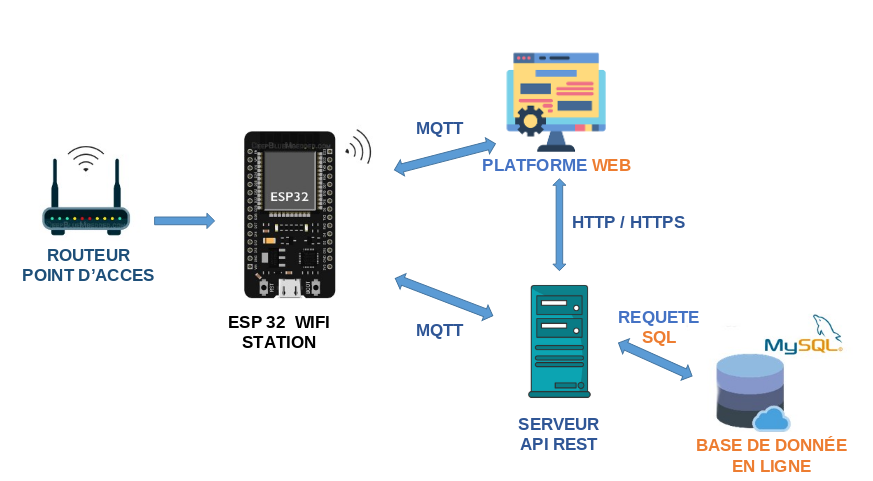
\includegraphics[width=17cm]{./img/composants/espWIFI.png}
	\caption{Utilisation WIFI intégrer au ESP32}
	\label{fig:moduleGSM1}
\end{figure}

\textbf{Fonctionnement} : \\
L'ESP32 se connecte à Internet via un routeur WiFi, qui joue le rôle de passerelle entre l'ESP32 et le serveur web. Les données sont échangées entre la plateforme et l'ESP32 à l'aide du protocole MQTT, tandis que le serveur web utilise une API REST pour interagir avec une base de données MySQL. Cette dernière stocke et gère les informations collectées pour permettre leur consultation ou mise à jour.


\subsection{Le module GSM pour l'envoi des messages}
Connecté à l'ESP32, le module GSM permet de transmettre des alertes par SMS via le réseau cellulaire. Il est spécifiquement conçu pour informer l'utilisateur en cas de dépassement de seuils critiques, tels qu'une tension trop faible ou une surchauffe.\\

\begin{figure}[H]
	\centering
	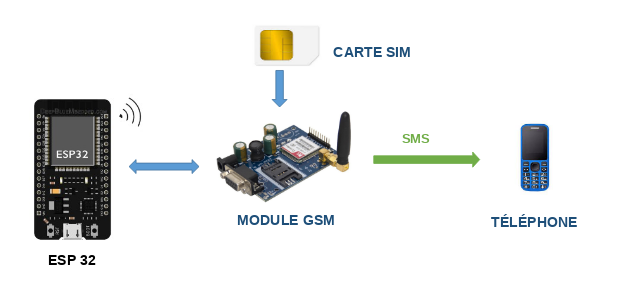
\includegraphics[width=15cm]{./img/composants/espGSM1.png}
	\caption{Module GSM pour la transmission}
	\label{fig:moduleGSM}
\end{figure}

L'image \ref{fig:moduleGSM} montre un système de communication utilisant un module GSM pour envoyer des SMS d'alerte.

\textbf{Processus de fonctionnement :}
\begin{enumerate}
	\item \textbf{Carte SIM :} Insérée dans le module GSM pour accéder au réseau cellulaire.
	\item \textbf{Module GSM :} Reçoit des données d'un ESP32 chargé de les collecter.
	\item \textbf{Envoi de SMS :} Le module envoie des SMS d'alerte en cas de dépassement de seuils critiques.
\end{enumerate}

\textbf{Résumé :}  
L'ESP32 envoie des alertes au module GSM, qui les transmet sous forme de SMS en cas de dépassement de seuils critiques.

%\subsection{Le module GSM pour la transmission des données} Connecté à l'ESP32, le module GSM permet de transmettre les données via le réseau cellulaire. Il envoie des requêtes HTTP pour les mises à jour, et peut également transmettre des SMS d'alerte en cas de dépassement de seuils critiques (tension trop faible, surchauffe, etc.).\\

%L'image \ref{fig:moduleGSM} montre un système de communication utilisant un module GSM pour transmettre des données à une base de données via un serveur API REST.

%\textbf{Processus de fonctionnement :}
%\begin{enumerate}
%	\item \textbf{Carte SIM :} Insérée dans le module GSM pour accéder au réseau cellulaire.
%	\item \textbf{Module GSM :} Reçoit des données d'un ESP32 chargé de les collecter.
%	\item \textbf{Transmission GSM :} Le module envoie les données via le réseau cellulaire vers un serveur API REST.
%	\item \textbf{Serveur API REST :} Reçoit, interprète et traite les données.
%	\item \textbf{Requête SQL :} Le serveur envoie ensuite une requête SQL pour insérer les données dans la base de données.
%	\item \textbf{Base de données :} Stocke les données pour un accès et une analyse ultérieure.
%	\item \textbf{Notification par SMS :} Le module peut aussi envoyer des SMS à un téléphone mobile.
%\end{enumerate}

%\begin{figure}[H]
%	\centering
%	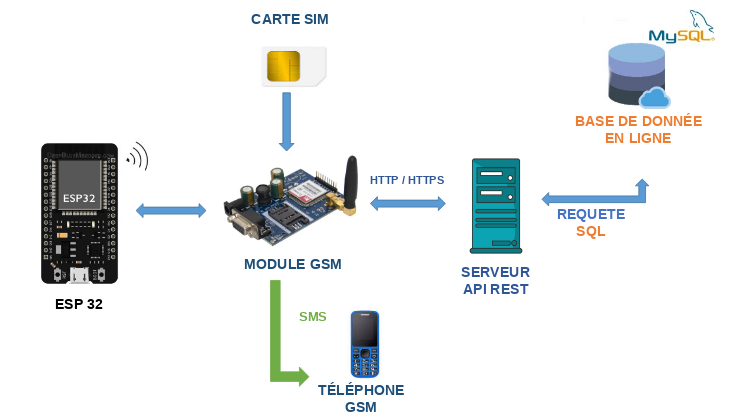
\includegraphics[width=17cm]{./img/composants/espGSM.png}
%	\caption{Module GSM pour la transmission}
%	\label{fig:moduleGSM}
%\end{figure}


%\textbf{Résumé :}  
%L'ESP32 envoie les données au module GSM, qui les transmet au serveur API REST pour traitement et stockage dans la base de données. Des SMS peuvent également être envoyés.

\subsection{Réseaux Wi-Fi }
Le \textbf{Wi-Fi} est une technologie de réseau sans fil qui utilise des fréquences radio dans les bandes de 2,4 GHz et 5 GHz pour fournir une connectivité Internet et des réseaux locaux. Elle permet la communication entre les appareils sans nécessiter de câbles, en utilisant des points d'accès (routeurs) pour transmettre les données via des ondes radio.

\subsubsection*{Fréquences}
\begin{itemize}
	\item \textbf{2,4 GHz} : Plus ancien, avec une portée plus longue mais une bande passante plus limitée et une plus grande congestion due à l'utilisation par d'autres appareils comme les téléphones sans fil et les micro-ondes.
	\item \textbf{5 GHz} : Moins encombré et offrant des vitesses de transmission plus élevées, mais avec une portée plus courte.
\end{itemize}

\subsubsection*{Débit}
Jusqu'à \textbf{600 Mbps} : débit maximal théorique selon les normes Wi-Fi, comme Wi-Fi 4 (802.11n), mais les versions plus récentes comme Wi-Fi 5 (802.11ac) et Wi-Fi 6 (802.11ax) offrent des débits beaucoup plus élevés.

\subsubsection*{Portée}
Environ \textbf{35 mètres} : portée typique en intérieur, réduite par les obstacles comme les murs épais.

\subsubsection*{Protocole}
Le Wi-Fi est un protocole \textbf{bidirectionnel}, permettant à la fois l'envoi et la réception de données, essentiel pour la mise à jour des micrologiciels et la communication entre appareils.
\subsubsection*{Avantages}
\begin{itemize}
	\item \textbf{Grande couverture} : adapté aux environnements nécessitant une large couverture, comme les bâtiments et espaces publics.
	\item \textbf{Haute vitesse} : les normes récentes (Wi-Fi 5, Wi-Fi 6) offrent des vitesses élevées, idéales pour le transfert de grandes quantités de données.
	\item \textbf{Interopérabilité} : le Wi-Fi est largement utilisé et compatible avec divers appareils et réseaux.
	\item \textbf{Coût réduit} : solution économique par rapport à d'autres protocoles sans fil.
	\item \textbf{Efficacité énergétique} : les dernières normes améliorent la gestion de l'énergie pour les dispositifs IoT.
	\item \textbf{Sécurité renforcée} : normes comme WPA3 garantissent une meilleure protection des données.
\end{itemize}


Le Wi-Fi est une technologie de communication sans fil robuste et flexible, offrant une connectivité rapide, fiable et sécurisée pour les réseaux IoT. Sa capacité à couvrir de grandes zones, sa vitesse élevée et ses fonctionnalités de sécurité en font une solution idéale pour cet projet.
\subsection{Réseau cellulaire GSM}

Le \textbf{GSM} est une norme de communication cellulaire largement utilisée pour la téléphonie mobile et les communications de données, fonctionnant sur les bandes de fréquences 900 MHz et 1800 MHz en Europe, ainsi que 850 MHz et 1900 MHz dans d'autres régions. Il offre une couverture étendue, permettant aux appareils de communiquer efficacement dans des zones urbaines et rurales.

Dans ce projet, le GSM est utilisé exclusivement pour envoyer des messages d'alerte en cas de dépassement de seuils critiques, tels qu'une tension trop faible ou une surchauffe. Grâce à sa fiabilité, le GSM garantit que les alertes par SMS parviennent à l'utilisateur, même dans des zones éloignées où d'autres options de connectivité peuvent être limitées.

\subsection*{Avantages}
\begin{itemize}
	\item \textbf{Couverture mondiale} : idéal pour les applications IoT nécessitant une portée étendue.
	\item \textbf{Interopérabilité} : compatible avec divers équipements dans différents pays.
	\item \textbf{Coût faible} : économique pour l'envoi de messages d'alerte.
	\item \textbf{Fiabilité} : technologie mature et éprouvée.
\end{itemize}

\subsection*{Inconvénients}
\begin{itemize}
	\item \textbf{Débit limité} : inadapté aux applications nécessitant des débits élevés.
	\item \textbf{Obsolescence} : en déclin avec la montée des réseaux 4G/5G.
\end{itemize}

L'utilisation du GSM dans ce projet de monitoring assure une communication fiable et économique, renforçant la capacité de surveiller les batteries solaires efficacement.

\subsection{Le protocole MQTT}  
Le protocole Message Queuing Telemetry Transport est un protocole de messagerie léger conçu pour les systèmes à ressources limitées et les communications dans des environnements où la bande passante réseau est restreinte. Il est particulièrement adapté aux applications IoT (Internet of Things) et aux dispositifs connectés nécessitant des échanges efficaces et rapides de données.  

\subsubsection{Caractéristiques principales de MQTT :}  
Le protocole MQTT repose sur le modèle \textbf{publish/subscribe (pub/sub)}, qui offre une communication flexible et asynchrone :  
\begin{itemize}  
	\item  \textbf{Publisher}  (émetteur) : envoie des messages à un ou plusieurs \textbf{topics} (sujets) spécifiques, sans se soucier des abonnés.  
	\item \textbf{Subscriber} (abonné) : s'inscrit à un ou plusieurs \textbf{topics} pour recevoir les messages publiés sur ces derniers.  
	\item \textbf{Broker} (serveur intermédiaire): joue un rôle central en agissant comme un médiateur entre les publishers et les subscribers. Il gère les abonnements, filtre les messages et distribue ceux-ci uniquement aux abonnés concernés.  


Pour la mise en œuvre, j’ai utilisé le broker open source \textbf{Mosquitto} [19], reconnu pour sa fiabilité, sa légèreté et sa compatibilité avec de nombreuses plateformes.  

\begin{figure}[H]
	\centering
	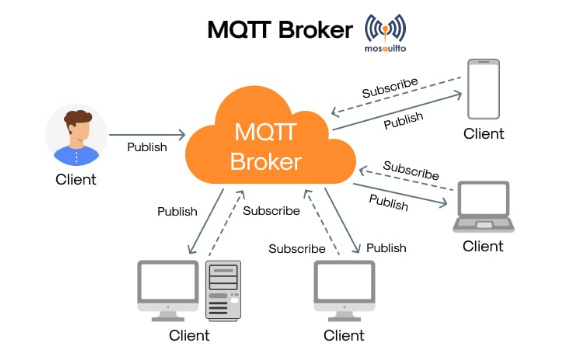
\includegraphics[width=14cm]{./img/broker.png}
	\caption{Le protocol MQTT}

\end{figure}


 	\item \textbf{Faible consommation de bande passante :}
MQTT utilise des paquets de données légers, ce qui le rend idéal pour les appareils avec une connexion réseau limitée.
\end{itemize}  
\subsection{Structure du protocole HTTP/HTTPS}

Le protocole HTTP/HTTPS repose sur un modèle client-serveur et se décompose en plusieurs éléments clés.

\subsubsection{Modèle requête-réponse}
Le protocole HTTP fonctionne selon un modèle requête-réponse, où le client envoie une requête au serveur, qui répond avec une réponse.

\subsubsection*{Requête HTTP}
Une requête HTTP se compose de trois parties :
\begin{itemize}
	\item \textbf{Ligne de requête} : contient la méthode (GET, POST, etc.), l'URL et la version du protocole. Exemple : \texttt{GET /index.html HTTP/1.1}.
	\item \textbf{En-têtes de requête} : métadonnées sur la requête. Exemple :
	\begin{verbatim}
	Host: www.example.com
	User-Agent: Mozilla/5.0
	\end{verbatim}
	\item \textbf{Corps de la requête} (facultatif) : utilisé pour les méthodes POST ou PUT. Exemple : \texttt{name=John\&age=25}.
\end{itemize}

\subsubsection*{Réponse HTTP}
Une réponse du serveur se divise en trois parties :
\begin{itemize}
	\item \textbf{Ligne de statut} : indique le résultat de la requête. Exemple : \texttt{HTTP/1.1 200 OK}.
	\item \textbf{En-têtes de réponse} : informations sur la réponse. Exemple :
	\begin{verbatim}
	Content-Type: text/html
	\end{verbatim}
	\item \textbf{Corps de la réponse} (facultatif) : contient les données demandées. Exemple :
	\begin{verbatim}
	<html><body>Welcome!</body></html>
	\end{verbatim}
\end{itemize}

\subsubsection{Méthodes HTTP}
Les principales méthodes incluent :
\begin{itemize}
	\item \textbf{GET} : récupérer une ressource.
	\item \textbf{POST} : envoyer des données au serveur.
	\item \textbf{PUT} : mettre à jour ou créer une ressource.
	\item \textbf{DELETE} : supprimer une ressource.
\end{itemize}

\subsubsection{Codes de Statut HTTP}
Les codes de statut indiquent le résultat de la requête :
\begin{itemize}
	\item \textbf{2xx (Succès)} : l'opération a réussi (ex. : 200 OK).
	\item \textbf{3xx (Redirection)} : la ressource a été déplacée (ex. : 301 Moved Permanently).
	\item \textbf{4xx (Erreur du client)} : la requête contient une erreur (ex. : 404 Not Found).
	\item \textbf{5xx (Erreur du serveur)} : le serveur a rencontré un problème (ex. : 500 Internal Server Error).
\end{itemize}

\subsubsection{HTTPS}
HTTPS est la version sécurisée de HTTP, utilisant TLS/SSL pour :
\begin{itemize}
	\item \textbf{Chiffrement} : cryptage des données échangées.
	\item \textbf{Authentification} : identification du serveur via un certificat SSL.
\end{itemize}

\subsubsection{Sessions et cookies}
HTTP est sans état, chaque requête étant indépendante. Les sessions sont gérées par des cookies, permettant de conserver des informations comme l'identifiant d'utilisateur.

\newpage
\section{ Modélisation de l'application web}
\subsection{Introduction}

Il est essentiel de modéliser les interactions entre les composants du système et les différents acteurs. À travers l'utilisation de diagrammes tels que le diagramme de cas d'utilisation, le diagramme d'activité et le diagramme de séquence, nous formaliserons le comportement, les interactions et la structure de l'application. Cette démarche vise à mieux comprendre l'architecture de l'application et à faciliter son développement.

\subsection{UML}
UML (Unified Modeling Language) est un langage standard pour modéliser les systèmes logiciels. Il propose divers diagrammes, comme le diagramme de cas d'utilisation pour représenter les interactions entre les acteurs et le système, le diagramme de séquence pour illustrer l'ordre des opérations, et le diagramme d'activité pour décrire les flux de processus. Ces outils permettent une conception claire et structurée, facilitant le développement et la maintenance des applications.
\subsubsection{Diagramme de cas d'utilisation}
Ce diagramme illustre les interactions entre les acteurs et le système, permettant de définir les fonctionnalités principales et les besoins des utilisateurs.

\begin{figure}[H]
	\centering
	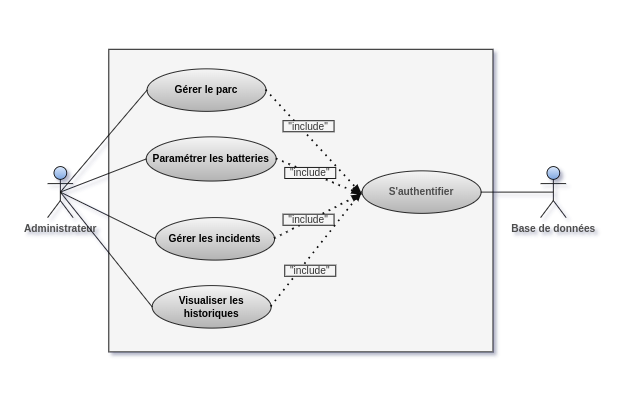
\includegraphics[width=17cm]{./img/composants/diagramme/Casutilisation.png}
	\caption{Diagramme de cas d'utilisation pour l'administrateur}
\end{figure}

\subsubsection{Diagramme d'activité}
Il décrit les flux de processus sous forme d'étapes successives et de décisions, utile pour modéliser les processus métier et les scénarios complexes.
\begin{figure}[H]
	\centering
	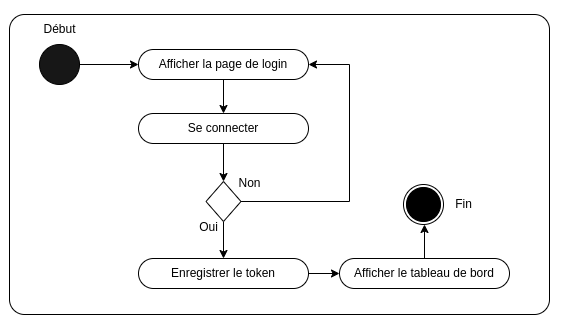
\includegraphics[width=16cm]{./img/composants/diagramme/auth.png}
	\caption{Diagramme d'activité pour l'authentification}
\end{figure}

\begin{figure}[H]
	\centering
	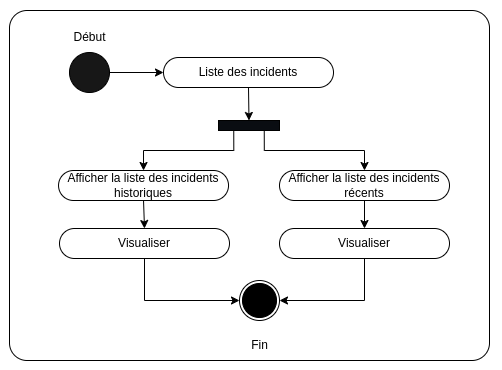
\includegraphics[width=14cm]{./img/composants/diagramme/Activiter-incident.png}
	\caption{Diagramme d'activité pour la gestion de la liste des incidents}
\end{figure}
\begin{figure}[H]
	\centering
	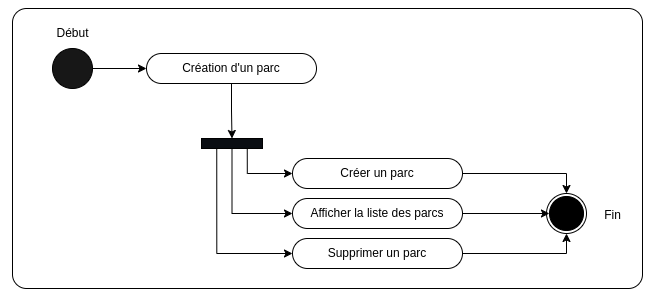
\includegraphics[width=16cm]{./img/composants/diagramme/creationParc.png}
	\caption{Diagramme d'activité pour la création de parc}
\end{figure}

\begin{figure}[H]
	\centering
	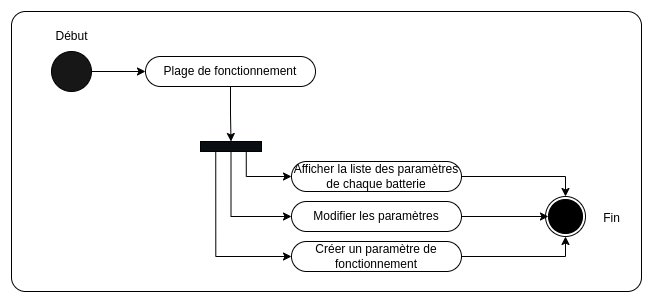
\includegraphics[width=16cm]{./img/composants/diagramme/Activiter-plagefonctionnement.png}
	\caption{Diagramme d'activité pour la plage de fonctionnement}
\end{figure}

\begin{figure}[H]
	\centering
	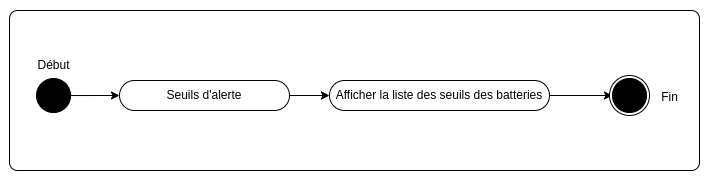
\includegraphics[width=16cm]{./img/composants/diagramme/Activiter-seuilesAlerte.png}
	\caption{Diagramme d'activité pour le seuil d'alerte}
\end{figure}

\begin{figure}[H]
	\centering
	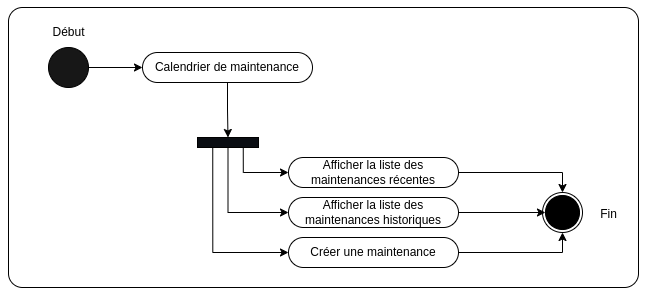
\includegraphics[width=16cm]{./img/composants/diagramme/Activiter-calendrier.png}
	\caption{Diagramme d'activité pour le calendrier de maintenance}
\end{figure}

\begin{figure}[H]
	\centering
	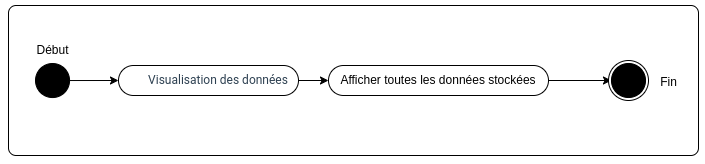
\includegraphics[width=16cm]{./img/composants/diagramme/Activiter-visualisation.png}
	\caption{Diagramme d'activité pour la visualisation des données}
\end{figure}








\subsubsection{Diagramme de séquence}
Ce diagramme montre l'ordre des messages échangés entre les composants ou objets d’un système, mettant en évidence la chronologie des interactions.

\begin{figure}[H]
	\centering
	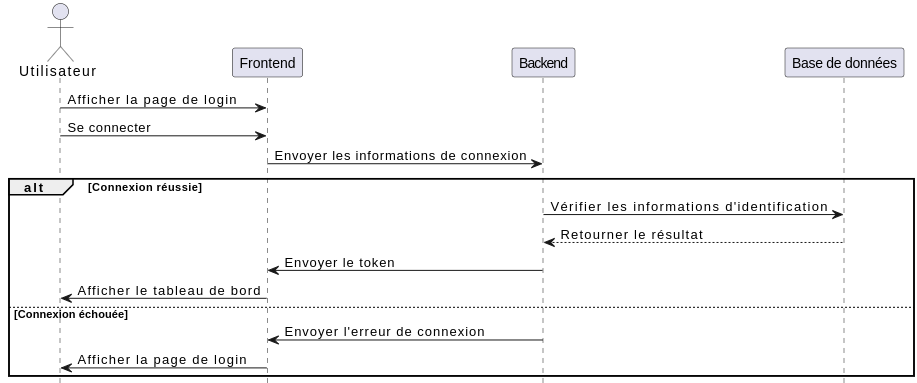
\includegraphics[width=17cm]{./img/composants/diagramme/seq/1-seq-auth.png}
	\caption{Diagramme de séquence pour l'authentification}
\end{figure}


\begin{figure}[H]
	\centering
	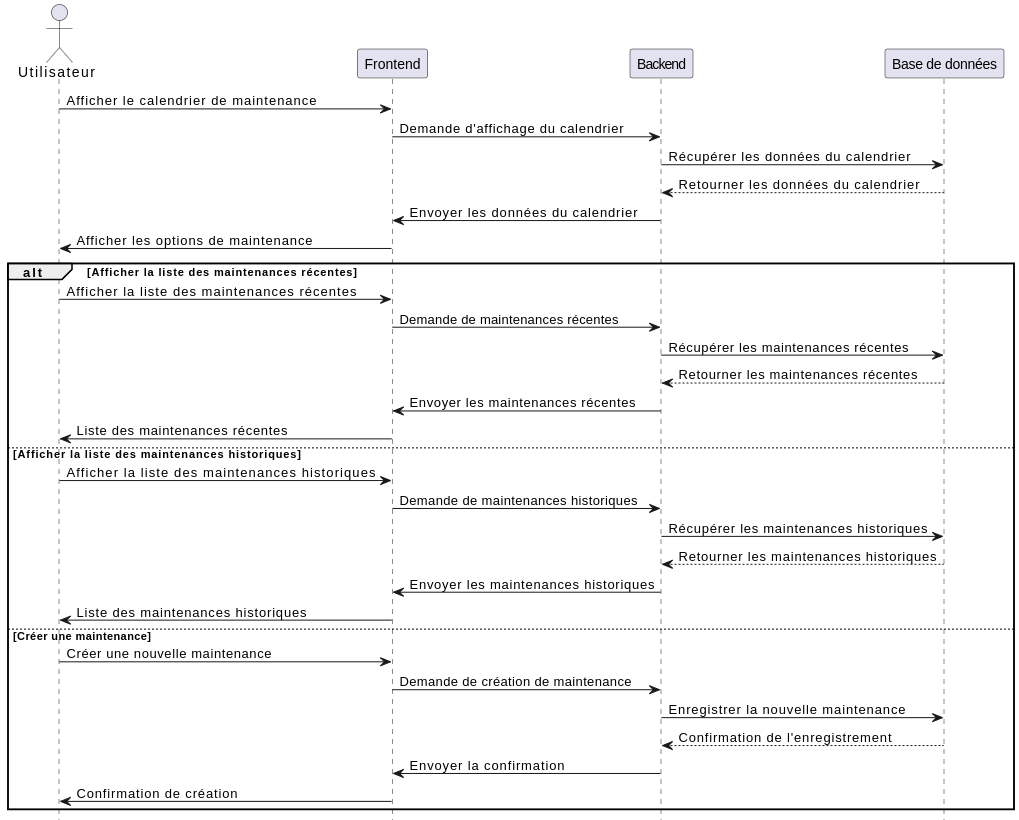
\includegraphics[width=16cm]{./img/composants/diagramme/seq/2sequeMaintenance.png}
	\caption{Diagramme de séquence pour le calendrier de maintenance}
\end{figure}
\begin{figure}[H]
	\centering
	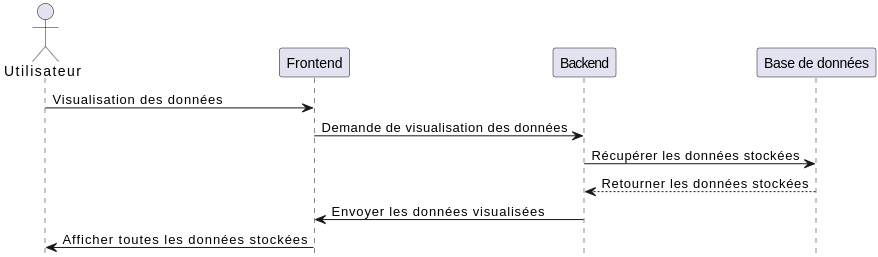
\includegraphics[width=17cm]{./img/composants/diagramme/seq/5seqvisualisation.png}
	\caption{Diagramme de séquence pour la visualisation des données}
\end{figure}
\begin{figure}[H]
	\centering
	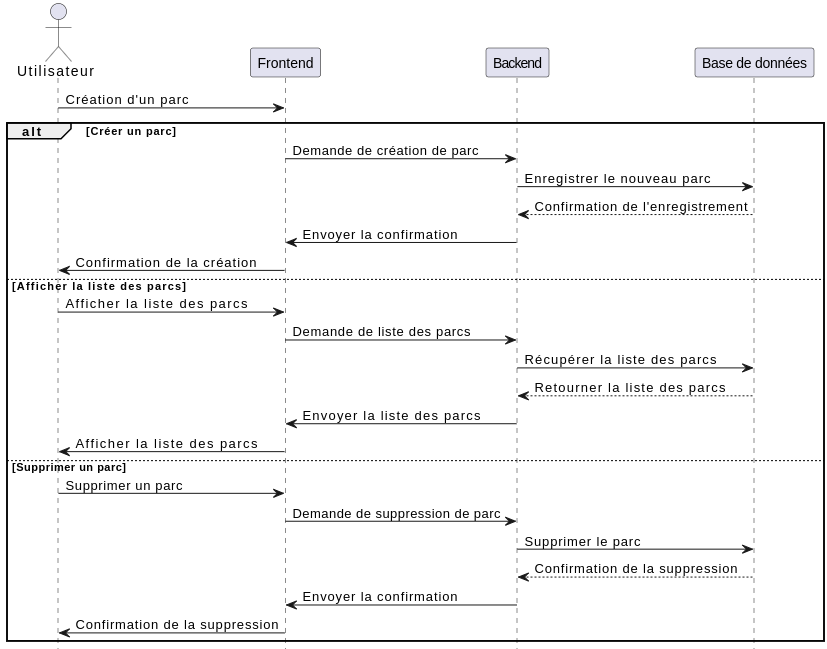
\includegraphics[width=15cm]{./img/composants/diagramme/seq/parc.png}
	\caption{Diagramme de séquence pour la création de parc}
\end{figure}
\begin{figure}[H]
	\centering
	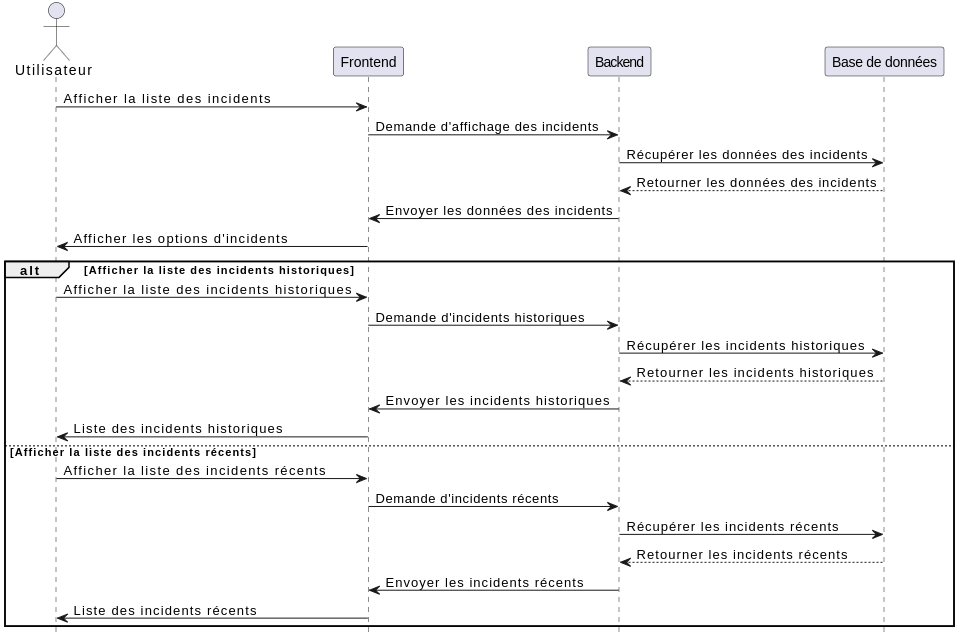
\includegraphics[width=15cm]{./img/composants/diagramme/seq/3seqyIncidentdrawio.png}
	\caption{Diagramme de séquence pour la gestion de la liste des incidents}
\end{figure}

\begin{figure}[H]
	\centering
	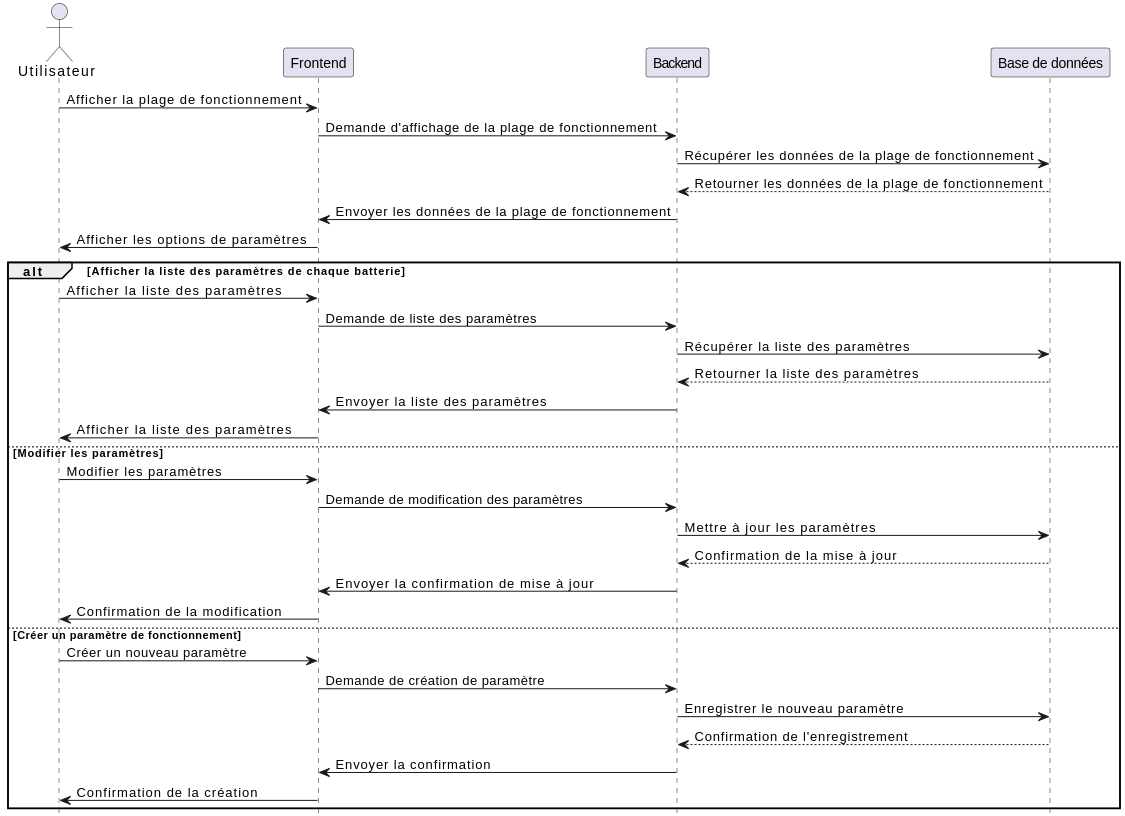
\includegraphics[width=15cm]{./img/composants/diagramme/seq/4seqplagefon.png}
	\caption{Diagramme de séquence pour la plage de fonctionnement}
\end{figure}
\begin{figure}[H]
	\centering
	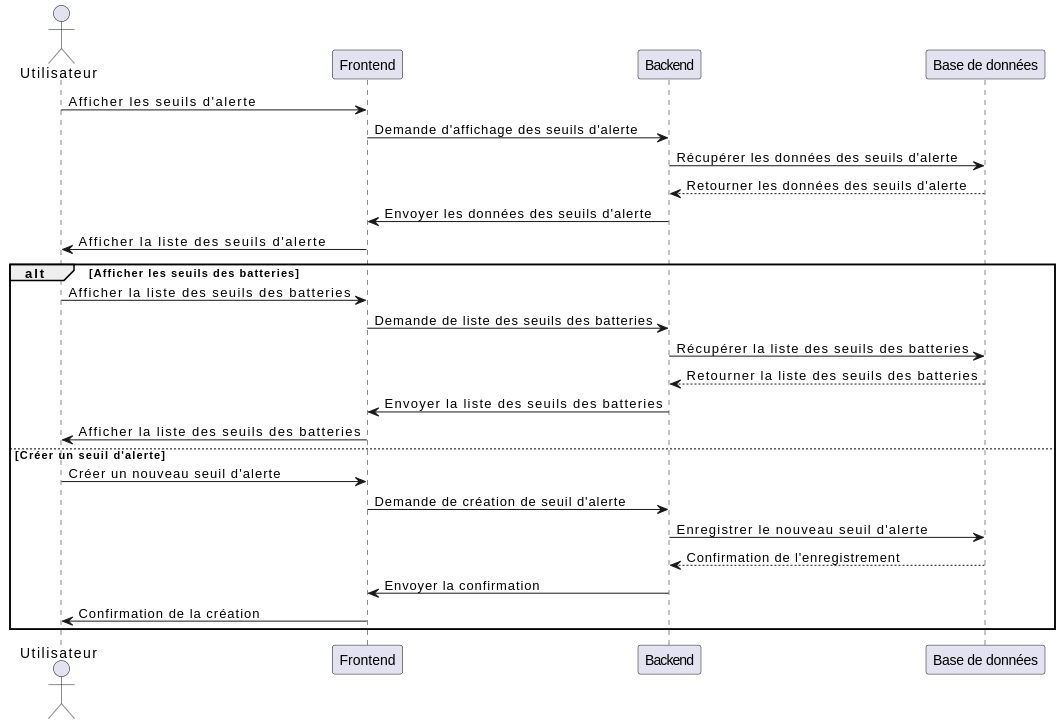
\includegraphics[width=15cm]{./img/composants/diagramme/seq/seuil.png}
	\caption{Diagramme de séquence pour le seuil des batteries}
\end{figure}
\begin{figure}[H]
	\centering
	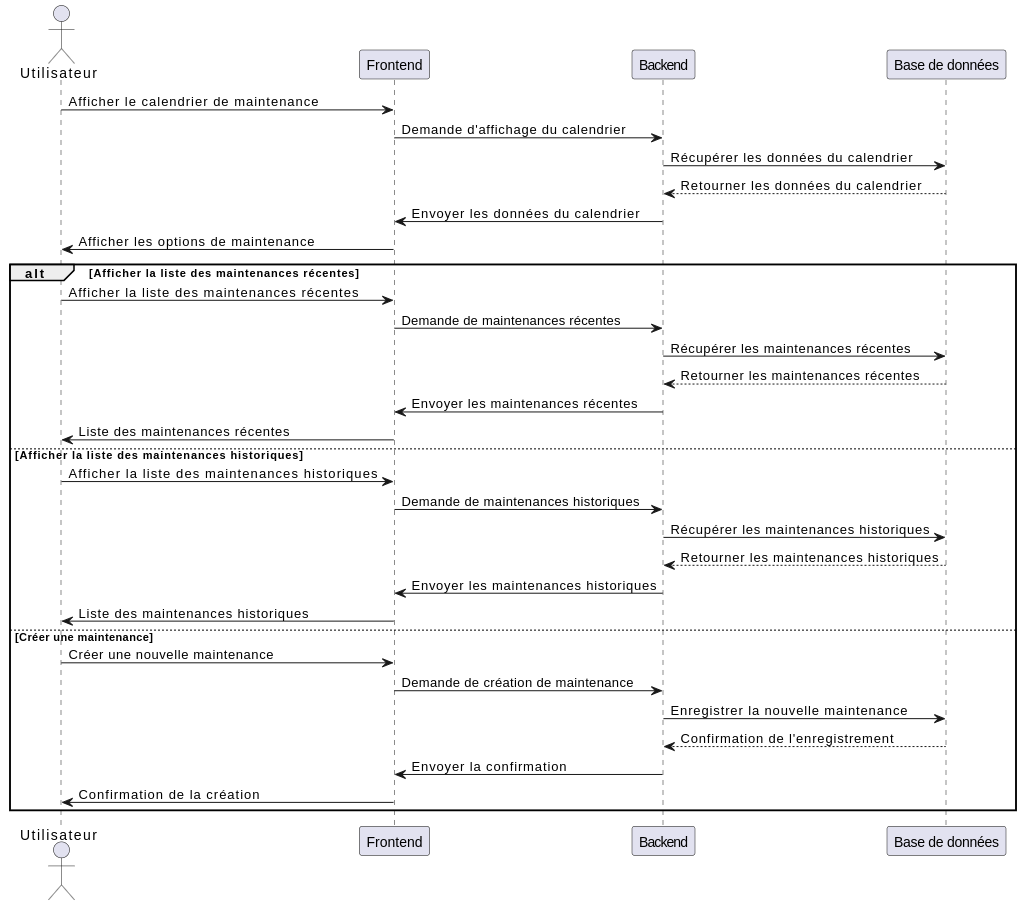
\includegraphics[width=17cm]{./img/composants/diagramme/seq/calendrier.png}
	\caption{Diagramme de séquence pour la calendrier de maintenance}
\end{figure}

\subsubsection{Diagramme de classe}

Un diagramme de classe UML est une représentation graphique qui illustre la structure statique d'un système. Il modélise les classes, leurs attributs, leurs méthodes (ou opérations) et les relations qui les lient.

\begin{itemize}
	\item \textbf{Nom de la classe} : il identifie la classe et se trouve dans le compartiment supérieur.
	\item \textbf{Attributs} : ce sont les propriétés ou caractéristiques d'une classe. Ils sont définis par leur visibilité, leur nom et leur type, et se placent dans le compartiment central. \\
	Exemple : \texttt{[visibilité] nomAttribut : type}.
	\item \textbf{Méthodes} : elles décrivent les comportements ou fonctionnalités d'une classe, définies par leur visibilité, leur nom, leurs paramètres et leur type de retour.
	\item \textbf{Visibilités} :
	\begin{itemize}
		\item \texttt{+} : Public,
		\item \texttt{-} : Privé,
		\item \texttt{\#} : Protégé.
	\end{itemize}
	\item \textbf{Relations} :
	\begin{itemize}
		\item \textbf{Association} : un lien entre deux classes, indiquant une interaction. La cardinalité précise le nombre d'instances impliquées (ex. : \texttt{1, 0..*, etc.}).
		\item \textbf{Héritage} : une relation où une classe dérivée hérite des propriétés et méthodes d'une classe parent.
		\item \textbf{Composition} : une relation forte où une classe fait partie intégrante d'une autre.
		\item \textbf{Agrégation} : une relation plus flexible où une classe est associée à une autre mais peut exister de façon indépendante.
		\item \textbf{Implémentation} : une classe dérivée implémente une interface.
	\end{itemize}
\end{itemize}

Dans ce projet, les diagrammes de classe ont été réalisés avec l'outil \textbf{PlantUML}, qui utilise une syntaxe textuelle simple pour créer des diagrammes. À noter que, dans PlantUML, la visibilité publique (représentée par \texttt{+} en UML standard) est affichée sous forme d'un petit rond.

Pour ce travail, les outils \textbf{UML Designer} et \textbf{PlantUML} ont été utilisés pour générer les diagrammes UML [27] [28].

\textbf{NB} : Le diagramme de classe final est présenté en annexe, au format A3.








\subsection{Draw.io}

Pour la modélisation, le logiciel libre ``Draw.io'' a été utilisé pour dessiner le diagramme de classe.

\section{Conclusion}

Dans ce chapitre, nous avons détaillé la transmission des données en utilisant le module GSM. Nous avons également abordé le protocole HTTP/HTTPS, qui s'est révélé être une solution fiable et sécurisée pour notre projet. Les données transmises sont ensuite stockées dans une base de données en ligne via une API REST, pour laquelle nous avons structuré la base afin d'assurer une gestion optimale des informations. Le prochain chapitre sera consacré à la réalisation pratique du dispositif, avec un focus sur les interfaces, les connexions et le schéma global du système.
